\section{Experiments}\label{sec:experiments}

\subsection{Set-Up}

All runs used one RTX 5080 GPU (16 GB). Seeds are stated in the table captions; the gradient-boosting baselines (GBM) use scikit-learn~\cite{pedregosa2011sklearn}. Macro-F1 is in percent under the protocols of Section~\ref{sec:dataset}; the headline is the drive level on held-out car models, scored once per final model after all choices had been made on the internal folds. Unit-level intervals are 95\% cluster bootstraps over car models (with several seeds, the mean of the seeds' bounds); multi-seed entries are mean $\pm$ std.

\subsection{Main Results on Held-Out Car Models}

Table~\ref{tab:main} gives the headline results. Architecture is not the bottleneck: the four reference sequence models lie within about 2 points at window level and close together at drive level. Averaging the windows of a drive adds 7--12 points; pooling further to vehicle level does not. For the sequence models, windows without automation activity (human-only columns) are harder for size and easier for BEV vs ICE, which Section~\ref{sec:discussion} relates to the controller of the driving automation system (DAS); the human-only drive columns cover fewer drives and are not directly comparable with the full columns.

\begin{table*}[t]
\centering
\footnotesize
\setlength{\tabcolsep}{3.2pt}
\caption{Held-out car models (\texttt{split\_platform} test split; size / BEV vs ICE: 41 / 39 car models, 1,141 / 836 drives, 732 / 564 with human-only windows, 329 / 244 vehicles). Macro-F1 in percent (protocols of Section~\ref{sec:dataset}); deep models mean over three seeds (std where given), GBM single-seed; chance about 33 (size) and 50 (BEV vs ICE). S9 / B5: recipes selected on the internal folds (Section~\ref{sec:methods}); episode MIL with window-mean aggregation and its own bag prediction; bootstrap intervals in the text.}
\label{tab:main}
\begin{tabular}{@{}lcccccccccc@{}}
\toprule
 & \multicolumn{5}{c}{Size (SMALL / MID / LARGE)} & \multicolumn{5}{c}{BEV vs ICE} \\
\cmidrule(lr){2-6} \cmidrule(lr){7-11}
 & \multicolumn{2}{c}{window} & \multicolumn{2}{c}{drive} & vehicle & \multicolumn{2}{c}{window} & \multicolumn{2}{c}{drive} & vehicle \\
\cmidrule(lr){2-3} \cmidrule(lr){4-5} \cmidrule(lr){6-6} \cmidrule(lr){7-8} \cmidrule(lr){9-10} \cmidrule(lr){11-11}
Model & full & human & full & human & full & full & human & full & human & full \\
\midrule
Statistics + GBM & 49.7 & 46.3 & 54.7 & 50.5 & 51.5 & 69.5 & 73.5 & 73.2 & 74.3 & 76.0 \\
LLM features + GBM & 40.5 & 47.3 & 63.2 & 58.9 & 58.6 & 69.6 & 84.2 & 89.4 & 89.1 & 90.1 \\
LLM + statistics + GBM & 54.1 & 49.8 & 64.9 & 64.2 & 61.8 & 73.2 & 80.2 & 80.9 & 82.6 & 83.4 \\
\midrule
1-D ResNet & 53.6 $\pm$ 1.0 & 48.0 & 61.1 $\pm$ 1.3 & 60.3 & 56.4 & 78.4 $\pm$ 0.4 & 83.2 & 91.1 $\pm$ 0.8 & 89.5 & 90.3 \\
bi-GRU & 54.7 $\pm$ 0.3 & 50.4 & 62.9 $\pm$ 0.8 & 63.3 & 57.2 & 79.2 $\pm$ 0.8 & 85.2 & 89.0 $\pm$ 0.1 & 90.8 & 88.6 \\
Transformer & 52.5 $\pm$ 0.8 & 47.7 & 61.8 $\pm$ 0.9 & 61.3 & 55.3 & 77.0 $\pm$ 0.4 & 83.5 & 88.4 $\pm$ 0.6 & 90.1 & 89.0 \\
Mamba-2 (bidirectional) & 53.1 $\pm$ 0.4 & 49.8 & 61.2 $\pm$ 0.3 & 61.1 & 55.2 & 77.3 $\pm$ 0.7 & 84.0 & 89.4 $\pm$ 0.3 & 90.9 & 90.6 \\
\midrule
bi-GRU, S9 & 53.2 $\pm$ 0.3 & 47.8 & 67.1 $\pm$ 0.0 & 61.7 & 60.0 $\pm$ 0.6 & -- & -- & -- & -- & -- \\
1-D ResNet, S9 & 53.2 $\pm$ 0.8 & 49.5 & 66.8 $\pm$ 1.7 & 62.9 & 62.6 $\pm$ 1.4 & -- & -- & -- & -- & -- \\
bi-GRU, B5 & -- & -- & -- & -- & -- & 77.0 $\pm$ 0.3 & 83.7 & 92.6 $\pm$ 0.1 & 89.1 & 93.4 $\pm$ 0.4 \\
1-D ResNet, B5 & -- & -- & -- & -- & -- & 79.9 $\pm$ 0.7 & 83.2 & 93.0 $\pm$ 0.8 & 88.7 & 92.8 $\pm$ 0.4 \\
Episode MIL, window mean & 54.2 $\pm$ 0.3 & 50.0 & 64.6 $\pm$ 0.5 & 62.5 & 62.3 $\pm$ 0.9 & 78.8 $\pm$ 0.1 & 82.2 & 90.2 $\pm$ 0.2 & 89.9 & 90.4 $\pm$ 0.5 \\
Episode MIL, bag prediction & -- & -- & 64.3 & 63.2 & 62.4 & -- & -- & 93.0 & 91.5 & 92.8 \\
\bottomrule
\end{tabular}
\end{table*}

The recipes selected on the folds raise the drive level without a matching gain at window level: S9 adds 4--6 points on size and B5 2--4 points on BEV vs ICE over the reference GRU and ResNet. The gains are stable over seeds, but the intervals over car models overlap (GRU S9 67.1 [54.4, 74.2] against the reference GRU 62.9 [48.9, 72.4]; GRU B5 92.6 [87.1, 96.2] against 89.0 [81.8, 93.7]). The episode MIL model matches but does not beat the window recipes under either aggregation; its fold advantage on BEV vs ICE (95.8, Table~\ref{tab:folds}) did not carry to the test models.

\subsection{Held-Out Devices}

Table~\ref{tab:device} repeats the main rows with devices held out and car models shared: all drive-level scores are far higher and the LLM + statistics GBM becomes the best size model. The recipes appear to trade within-model recognition for cross-model generalisation, since GRU S9 is below the reference GRU at window level and slightly above it at drive level (79.5 [70.8, 84.4] against 78.1).

\begin{table}[t]
\centering
\footnotesize
\setlength{\tabcolsep}{3pt}
\caption{Held-out devices, car models shared (\texttt{split\_device} test split; size 1,218 drives / 219 vehicles / 81 car models, BEV vs ICE 922 / 143 / 63). Macro-F1 in percent per window and per drive (protocol full); mean $\pm$ std over three seeds, one seed for GBM and MIL.}
\label{tab:device}
\begin{tabular}{@{}lcccc@{}}
\toprule
 & \multicolumn{2}{c}{Size} & \multicolumn{2}{c}{BEV vs ICE} \\
\cmidrule(lr){2-3} \cmidrule(lr){4-5}
Model & window & drive & window & drive \\
\midrule
LLM + stat. + GBM & 72.4 & 80.6 & 84.4 & 94.1 \\
1-D ResNet & 68.4 $\pm$ 3.0 & 77.4 $\pm$ 2.2 & 82.4 $\pm$ 0.7 & 96.2 $\pm$ 0.5 \\
bi-GRU & 70.2 $\pm$ 0.9 & 78.1 $\pm$ 1.4 & 87.4 $\pm$ 0.4 & 96.5 $\pm$ 0.1 \\
ResNet S9 / B5 & 64.8 $\pm$ 0.3 & 80.6 $\pm$ 0.1 & 83.1 $\pm$ 0.2 & 97.2 $\pm$ 0.3 \\
GRU S9 / B5 & 62.9 $\pm$ 1.0 & 79.5 $\pm$ 0.7 & 78.8 $\pm$ 0.4 & 95.1 $\pm$ 0.3 \\
MIL (1 seed) & 68.4 & 78.8 & 86.5 & 96.1 \\
\bottomrule
\end{tabular}
\end{table}

\subsection{Internal Folds and Recipe Sweep}

Table~\ref{tab:folds} summarises the campaign on the internal folds of Section~\ref{sec:methods}. Gate G1 passed: the three-fold means of the reference recipe lie within about 5 points of its test values in Table~\ref{tab:main}. The fold-0 size sweep spans 4 points, no more than the spread between folds, and no recipe approaches 70, so gate G2 for size fails; on BEV vs ICE, augmentation (B4) brings the gain and B5 reaches 93.1 over three folds, passing G2. The episode MIL model with gated attention~\cite{ilse2018mil} is level with S9 on size (G3 fails) and +2.7 over B5 on BEV vs ICE (G3 passes); its window-mean aggregation is weaker (61.1 and 88.8), and gated attention beats a learned instance mean on fold 0 (67.8 against 66.7; 96.0 against 94.8).

The final models train for fixed epoch counts taken from the folds; their shared-model validation scores (GRU / ResNet S9 60.7 / 62.8 and B5 75.6 / 79.3; MIL 79.1 on size and 97.5 on BEV vs ICE) are no guide to the test values.

\begin{table}[t]
\centering
\footnotesize
\caption{Model-disjoint internal folds of Section~\ref{sec:methods}: drive-level macro-F1 (protocol full) on each fold's held-out car models and the three-fold mean, one seed per entry; MIL rows are the model's own bag prediction; S0 / B0 reference, S9 / B5 final recipes. (a) Fold-0 sweep with the bi-GRU; (b) candidates on all three folds.}
\label{tab:folds}
\setlength{\tabcolsep}{2.3pt}
\begin{tabular}{@{}lcccccccccc@{}}
\toprule
\multicolumn{11}{@{}l}{(a) Fold 0, bi-GRU} \\
\midrule
Size & S0 & S1 & S2 & S3 & S4 & S5 & S6 & S7 & S8 & S9 \\
 & 65.3 & 62.8 & 66.8 & 64.8 & 65.2 & 66.2 & 64.8 & 65.6 & 66.5 & 66.9 \\
\addlinespace
BEV vs ICE & B0 & B1 & B2 & B3 & B4 & B5 & & & & \\
 & 89.4 & 88.0 & 87.4 & 88.7 & 92.8 & 92.8 & & & & \\
\bottomrule
\end{tabular}
\par\smallskip
\setlength{\tabcolsep}{4pt}
\begin{tabular}{@{}lcccc@{}}
\toprule
\multicolumn{5}{@{}l}{(b) Three folds} \\
\midrule
Recipe & fold 0 & fold 1 & fold 2 & mean \\
\midrule
\multicolumn{5}{@{}l}{\emph{Size}} \\
GRU S0 (reference) & 65.3 & 69.5 & 60.4 & 65.1 \\
GRU S2 (footprint head) & 66.8 & -- & -- & 65.5 \\
GRU S5 (augmentation) & 66.2 & -- & -- & 66.5 \\
GRU S9 (final) & 66.9 & 70.5 & 64.8 & 67.4 \\
ResNet S0 (reference) & -- & -- & -- & 66.6 \\
ResNet S9 (final) & 67.0 & 70.4 & 61.2 & 66.2 \\
Episode MIL, bag & 67.8 & 65.6 & 67.5 & 67.0 \\
\addlinespace
\multicolumn{5}{@{}l}{\emph{BEV vs ICE}} \\
GRU B0 (reference) & 89.4 & 90.8 & 95.4 & 91.9 \\
GRU B4 (augmentation) & 92.8 & -- & -- & 92.8 \\
GRU B5 (final) & 92.8 & 91.1 & 95.4 & 93.1 \\
ResNet B0 (reference) & -- & -- & -- & 93.1 \\
ResNet B5 (final) & 95.7 & 93.9 & 96.1 & 95.2 \\
Episode MIL, bag & 96.0 & 98.2 & 93.2 & 95.8 \\
\bottomrule
\end{tabular}
\end{table}

\begin{figure}[t]
\centering
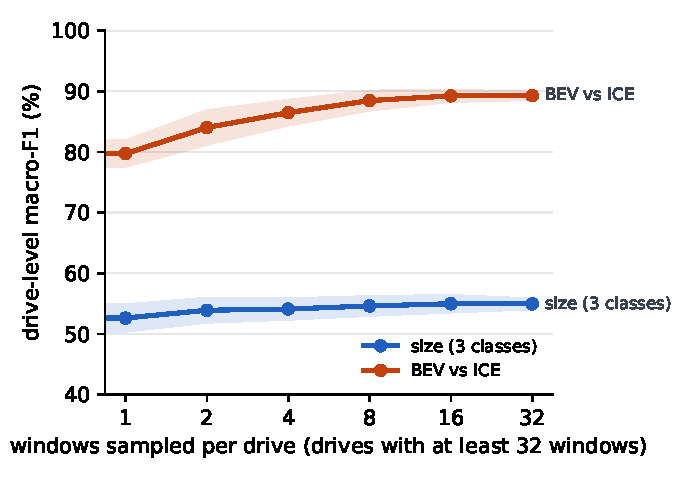
\includegraphics[width=0.85\columnwidth]{evidence_sufficiency.pdf}
\caption{Evidence sufficiency on held-out car models (reference predictions, drive-level macro-F1 in percent): on test drives with at least 32 eligible windows, $m$ windows are drawn per drive and their probability vectors averaged (mean over 50 draws; band: one std). Size moves from 52.6 ($m = 1$) to 54.9 ($m = 32$; all windows 56.0), BEV vs ICE from 79.7 to 89.3 (all windows 89.1), saturating by 8--16 windows.}
\label{fig:evidence}
\end{figure}

\subsection{Ceilings, Separability and Evidence Sufficiency}

Three zero-training oracles bound the size task on the held-out models: a per-car-model majority oracle (every drive of a held-out model gets that model's majority prediction) lifts the ensemble of the 12 reference deep runs from 63.2 to 72.0, so perfect within-model consistency would still leave size far from 90 (BEV vs ICE: 89.8 to 93.5). The footprint-noise oracle of Fig.~\ref{fig:ceiling} scores 92.1 at $\sigma = 0.10$ m$^2$ and 86.6 at 0.15, so reaching 90 needs a footprint error of about $\pm$0.12 m$^2$, about 2.5\% of a 4.6 m$^2$ footprint. A curb-mass oracle (two mass cuts fitted on the training drives) scores 63.3 on the 1,139 test drives with a known mass, so mass is no better proxy.

\begin{figure}[t]
\centering
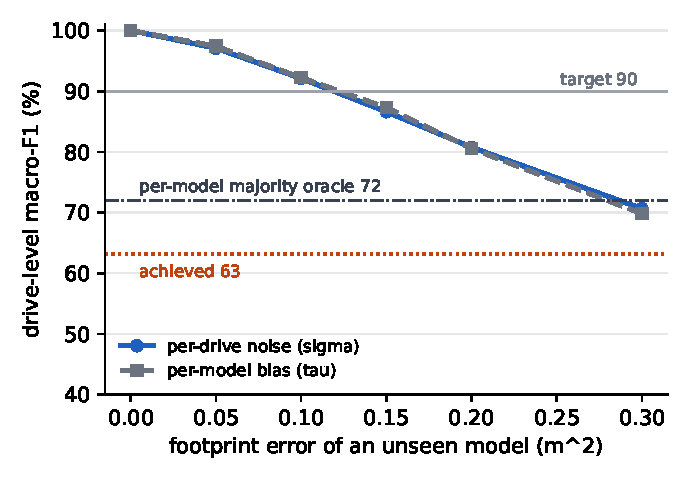
\includegraphics[width=0.85\columnwidth]{footprint_noise_oracle.pdf}
\caption{Footprint-noise oracle for the size task on held-out car models (drive-level macro-F1 in percent, 200 repeats): each drive is classified from the true footprint of its car model plus an error, cut at the fixed thresholds 4.43 and 4.88 m$^2$; per-drive noise of std $\sigma$ (circles) or a per-car-model bias $\tau$ (squares), both in m$^2$. Lines: the reference ensemble of the twelve reference sequence-model runs (63.2), its per-car-model majority oracle (72.0) and the 90 target.}
\label{fig:ceiling}
\end{figure}

The errors sit where the labels are closest: 21 of the 41 held-out car models lie within 0.15 m$^2$ of a differently labelled training model, and in one reference GRU run window accuracy is 53.0\% within 0.1 m$^2$ of a threshold against 89.9\% beyond 0.8 m$^2$. With the reference predictions, LARGE unibody vehicles are read as MID or SMALL while pickups and body-on-frame SUVs are recognised (per-model shares in Section~\ref{sec:discussion}), and MID models just above the 4.43 m$^2$ cut are read as SMALL (drives correct: GWM Haval H6, Audi Q5, Lexus RX and Nissan Altima 0\%, Kia Stinger 25\%).

Evidence per drive is not the limit for the reference models (Fig.~\ref{fig:evidence}): drive accuracy stays between 63.8 and 73.8\% (size) and 85.7 and 93.2\% (BEV vs ICE) from 1--2 to more than 64 windows per drive, and it does not grow with the number of acceleration, deceleration or lead-acceleration episodes.

\subsection{LLM-Proposed Physical Features}

Table~\ref{tab:llm} compares gradient boosting on hand-crafted window statistics, on the 34 registered LLM-proposed features and on both: alone, the physical features are weak per window but strong per drive, on a par with the reference sequence models on BEV vs ICE, and adding the statistics helps size but lowers BEV vs ICE at drive level. By permutation importance of the LLM-features-only gradient boosting on the validation split, BEV vs ICE rests on lift-off deceleration (while moving and shortly after pedal release), the share of deceleration under a pressed accelerator or without the brake, the lead-to-ego deceleration delay and the 10th percentile of brake-free deceleration; size on the curvature-per-steering-angle gain at 6--18 m/s and at low speed, the Ackermann gain at 6--12 m/s and the same delay.

\begin{table}[t]
\centering
\footnotesize
\setlength{\tabcolsep}{3.5pt}
\caption{Gradient boosting on window statistics, on the 34 registered LLM-proposed features and on both (held-out car models, one seed); macro-F1 in percent per window (full and human-only) and per drive (protocol full).}
\label{tab:llm}
\begin{tabular}{@{}lcccccc@{}}
\toprule
 & \multicolumn{3}{c}{Size} & \multicolumn{3}{c}{BEV vs ICE} \\
\cmidrule(lr){2-4} \cmidrule(lr){5-7}
Features & full & human & drive & full & human & drive \\
\midrule
Statistics & 49.7 & 46.3 & 54.7 & 69.5 & 73.5 & 73.2 \\
LLM physical & 40.5 & 47.3 & 63.2 & 69.6 & 84.2 & 89.4 \\
LLM + statistics & 54.1 & 49.8 & 64.9 & 73.2 & 80.2 & 80.9 \\
\bottomrule
\end{tabular}
\end{table}

\subsection{Aggregation and Ensembles}

Out of fold on the reference recipe (GRU and ResNet pooled), the best aggregation variant moves size from 67.5 to 67.8 (+0.3) and down-weighting DAS windows in the mean moves BEV vs ICE from 93.0 to 94.8 (+1.8), short of the pre-registered +1.0 on both tasks, so the plain mean remains the headline. Ensembles stayed below the G4 gate: a GRU + ResNet mean gains under one point over the best member out of fold (BEV vs ICE 93.9 against 93.1--93.5; size 68.8 against 68.2) and stacking is worse (92.3 and 66.5). The supplementary rule fixed before the final test run, the DAS- and episode-weighted log-odds mean of Section~\ref{sec:methods}, moves size from 66.9 to 68.7 on the six final S9 runs (+1.7, 6 of 6 runs improved) and BEV vs ICE from 92.8 to 93.5 on the six B5 runs (+0.7, 6 of 6).
